\chapter{Présentation générale}
\label{chap:Présentation générale}

% "*" makes the section unnumbered

\section*{Introduction}

\hspace{\parindent}Ce chapitre introduit notre rapport de projet de fin d'études. Nous commençons par présenter l'organisme d'accueil, B3G, en mettant en lumière ses solutions et sa clientèle. Ensuite, nous délimitons le cadre du projet et exposons la problématique à laquelle notre travail vise à répondre. Nous décrivons ensuite la solution proposée et les étapes de sa mise en œuvre. Enfin, nous abordons la conduite du projet, incluant le calendrier prévu et les étapes clés à venir. Cette introduction permet de comprendre le contexte global et de poser les bases pour la suite de notre rapport.
\newpage

\section{Présentation de l'entreprise}

\hspace{\parindent}Cette section présente l'organisme d'accueil du stage - B3G Tech, Omni Channel Digital Banking and Wallet.

\subsection{B3G Tech}

\hspace{\parindent}Fondée en 2004, B3G (cf. Figure 1) est une société de services spécialisée dans l'édition, l'intégration et l'optimisation de solutions digitales pour le secteur bancaire. Elle propose une solution omnicanale de banque digitale et de Mobile Money à travers sa suite d'applications intégrée, Fawri, qui permet une gestion unifiée de l'expérience client via divers canaux : Mobile, Web, SMS, Voix, Email et Kiosque.




%Use \paragraph{To start a paragraph}

\begin{figure}[H]
    \centering
    
\includegraphics[width=10cm]{Logos/B3G.png}
    \caption{B3G Digital Banking \& wallet}
    \label{fig:my_label} %Optional (If you want to reference the figure in later chapters)
\end{figure}

%[width=7cm] you control the size of the image. other options include: 
%[height=7cm] or [scale=0.5] (means half the size of the original image)


% Documentation: \href{https://www.overleaf.com/learn/latex/Inserting_Images}{Images}



% \begin{tabular}{ll}
%   First & Second \\
%   Third & Fourth
% \end{tabular}
% \\

% More complex table with borders:


% \begin{tabular}{|l|c|r|} \hline
%   Left aligned column & Centered column & Right aligned column \\ \hline
%   Text & Text & Text \\ \hline
% \end{tabular}
% \\

% Example of a short table

%{5cm} is the cell length, you can change it to suit your own table

\begin{table}[H]
    \centering
    \begin{tabular}{|m{5cm}|m{10cm}|}
        \hline
        Site web               & \href{https://b3gtech.com/}{B3G Tech } \\
        \hline
        Siège social           & Rabat                                  \\
        \hline
        Année de création      & 2004                                   \\
        \hline
        Type d'entreprise      & société privée / SARL                  \\
        \hline
        Taille de l'entreprise & 51-200 employés                        \\
        \hline
        Implantations          & Rabat, Casablanca, Paris               \\
        \hline
    \end{tabular}
    \caption{Fiche de l'entreprise}
\end{table}


% Example of a long table (that spans 2 pages or more), Latex will automatically split the table when it reaches the end of the page:

% \begin{longtable}[c]{| m{4.4cm} | m{11cm} |}
% \caption{Long table}\\
%  \hline

%  Cell & Description  \\ 
%  \hline
%  \endfirsthead

%  \hline

%  Cell & Description  \\ 
%  \hline
%  \endhead

%         \hline
%           Element11 & Element21 \\
%         \hline
%           Element12 & Element22 \\
%         \hline
%           Element13 & Element23 \\
%         \hline
%           Element14 & Element24 \\
%         \hline
%           Element15 & Element25 \\
%         \hline
%           Element16 & Element26 \\
%         \hline
%           Element17 & Element27 \\
%         \hline
%           Element18 & Element28 \\
%         \hline
%           Element19 & Element29 \\
%         \hline
%           Element110 & Element210 \\
%         \hline
%           Element111 & Element211 \\
%         \hline
%           Element112 & Element212 \\
%         \hline
%           Element113 & Element213 \\
%         \hline
%           Element114 & Element214 \\
%         \hline

%  \end{longtable}


% Documentation: \href{https://www.overleaf.com/learn/latex/Tables}{Tables}

\subsection{Produits \& Solutions}

\hspace{\parindent}B3G propose une gamme complète de solutions packagées regroupées sous la suite applicative FawriSuite. Cette suite Omnicanal offre une solution de Banque Digitale et Mobile Money entièrement intégrée, permettant de gérer de manière unifiée l'ensemble de l'expérience client à travers différents canaux tels que le mobile, le web, les SMS, la voix, l'e-mail et les kiosques. Parmi les solutions phares de la gamme FawriSuite, on retrouve FawriBank, FawriWallet et FawriAlert, qui couvrent respectivement les aspects de la banque digitale, du portefeuille électronique et des notifications transactionnelles.

FawriSuite, créée par B3G, est une plateforme informatique éprouvée destinée aux institutions financières, aux opérateurs de télécommunications, aux opérateurs de services publics et aux agences gouvernementales. Basée sur une Architecture Orientée Service (SOA), FawriSuite est une solution centrée sur le client, offrant flexibilité et visibilité à son expérience. Elle répond de manière personnalisée aux besoins spécifiques de chaque client à tous les points de contact.

La gamme FawriSuite propose des solutions packagées couvrant tous les aspects de la banque digitale :
\begin{itemize}
    \item \textbf{Fawri Bank}: Une solution Omnicanal intégrée de banque digitale offrant des services tels que l'E-Banking, le Mobile Banking, le SMS Banking, le Phone Banking, le Branch Banking et le Kiosk Banking, adaptée aux particuliers, professionnels et entreprises.
    \item \textbf{Fawri Wallet}: Une solution Core Banking \& Digitale front2back optimisée pour les comptes mobiles. Elle permet de gérer tout l'écosystème Mobile Money, y compris la gestion des agents et des commerçants, les fonctionnalités e-Commerce et le paiement mobile, favorisant ainsi l'inclusion financière et les stratégies CashLess.
    \item \textbf{Fawri Flow}:Une plate-forme Low-Code accélérant la digitalisation des processus, offrant ainsi une meilleure efficacité opérationnelle et une agilité accrue dans la transformation digitale des entreprises.


\end{itemize}



\begin{figure}[H]
    \centering
    
\includegraphics[width=3.5cm]{Logos/fawri.png}
    \caption{Fawri by B3G}
    \label{fig:my_label} %Optional (If you want to reference the figure in later chapters)
\end{figure}

\subsection{Clients de B3G}
\hspace{\parindent}B3G compte parmi ses clients de premier plan plusieurs institutions bancaires prestigieuses, notamment CIH Bank, Crédit Agricole du Maroc, BMCE Bank Of Africa, Umnia Bank,

LanaCash, et bien d'autres. En plus de ces institutions, B3G entretient des collaborations avec divers clients variés, tels que Veolia, Amendis et Dubai Plus.

\begin{figure}[H]
    \centering
    
\includegraphics[width=12cm]{Figures/clients.png}
    \caption{Clients de B3G}
    \label{fig:my_label} %Optional (If you want to reference the figure in later chapters)
\end{figure}

\subsection{B3G R\&D}

\hspace{\parindent}La division de recherche et développement de B3G se concentre avant tout sur la création de technologies qui permettront à B3G de rester à la pointe du secteur bancaire. Les chercheurs de B3G R\&D s'appuient sur des méthodologies et des approches innovantes, s'attaquant souvent à des défis ou des projets difficiles à réaliser au sein d'une organisation de développement de produits, ou impliquant un risque élevé ou une incertitude. La recherche de B3G R\&D se concentre sur des applications concrètes, et les chercheurs travaillent à la création de technologies qui auront un impact important sur l'évolution future de la société et de la technologie.

\section{Contexte général du projet}
\subsection{La transformation digitale des banques}

\hspace{\parindent}Le secteur bancaire a subi une transformation numérique remarquable ces dernières années, impulsée par les avancées technologiques, les évolutions des préférences des clients et les pressions concurrentielles. Cette métamorphose a radicalement modifié les modes opératoires des banques, leurs prestations de services et leurs interactions avec la clientèle.

\textbf{A. Évolution de la Banque Numérique :}

Traditionnellement, les opérations bancaires se déroulaient principalement dans des agences physiques, avec des processus manuels et des échanges en personne. Cependant, l'avènement des technologies numériques a métamorphosé les banques, les poussant à migrer des agences traditionnelles en dur vers des plateformes virtuelles.


\textbf{B. Facteurs de Transformation Numérique :}

Plusieurs éléments ont accéléré cette transformation dans le secteur bancaire :
\begin{itemize}
    \item \textbf{Attentes des Clients}: Les clients d'aujourd'hui exigent des expériences bancaires fluides, personnalisées et accessibles à tout moment et en tout lieu.
    \item \textbf{Concurrence}: L'émergence de start-ups fintech et de banques en ligne a intensifié la concurrence, incitant les banques traditionnelles à innover et à numériser leurs services.
    \item \textbf{Environnement Réglementaire}: Les changements réglementaires, notamment les initiatives de banque ouverte et les règles sur la protection des données, ont incité les banques à adopter des solutions numériques pour se conformer aux normes en évolution.
\end{itemize}


\textbf{C. Impact sur les Services Bancaires :}

La transformation numérique a entraîné des changements majeurs dans les services bancaires :
\begin{itemize}
    \item \textbf{Banque en ligne}: Les clients bénéficient désormais d'un large éventail de services bancaires en ligne, comme la gestion de compte, les paiements, les transferts de fonds et les demandes de prêt, via des plateformes sécurisées et des applications mobiles.
    \item \textbf{Expériences Personnalisées}: Les technologies d'analyse avancées et d'intelligence artificielle permettent aux banques de proposer des recommandations de produits sur mesure, des campagnes marketing ciblées et un service client proactif, améliorant ainsi l'expérience globale des clients.
    \item \textbf{Automatisation}: L'automatisation des processus manuels a conduit à une efficacité opérationnelle accrue, à des coûts réduits et à des délais de traitement plus rapides pour diverses transactions et services bancaires.
\end{itemize}



\subsection{Technologie Low-Code}

\hspace{\parindent}Les plates-formes de développement low-code occupent désormais une place centrale dans l'évolution de l'industrie logicielle, transformant fondamentalement la manière dont les applications sont conçues et déployées. Ces outils visuels facilitent la création, la modification et le déploiement d'applications même pour ceux qui ne possèdent pas de compétences en programmation, nécessitant très peu, voire aucun, codage.

En substance, ces plates-formes représentent un environnement de développement où les applications sont principalement configurées à l'aide d'interfaces graphiques plutôt que de lignes de code. Elles permettent aux utilisateurs de composer des applications à partir de composants préconstruits, en les reliant et en configurant les flux de travail de manière graphique.

\textbf{A. Les avantages du développement low-code :}

Les plateformes low-code sont précieuses, car elles rendent le développement accessible aux personnes qui n'ont pas forcément de compétences en codage, tout en permettant aux organisations de livrer des applications rapidement. Voici leurs principaux avantages :

\begin{itemize}
    \item \textbf{Rapidité}: Les outils low-code réduisent considérablement le temps nécessaire pour créer, prototyper, améliorer et déployer des applications, répondant ainsi aux exigences de rapidité de mise sur le marché, essentielles pour les entreprises.

    \item \textbf{Rentabilité }: Les plates-formes low-code élargissent l'accès au développement d'applications, permettant à un éventail plus large de personnes, y compris les non-programmeurs, de contribuer à la création d'applications, impliquant ainsi des profils tels que les analystes métier et les chefs de projet.

    \item \textbf{Accessibilité}: Les plates-formes low-code élargissent l'accès au développement d'applications, permettant à un éventail plus large de personnes, y compris les non-programmeurs, de contribuer à la création d'applications, impliquant ainsi des profils tels que les analystes métier et les chefs de projet.

    \item \textbf{Flexibilité et Agilité}: Grâce à leur nature modulaire, les plates-formes low-code offrent une grande flexibilité pour répondre rapidement aux besoins changeants, permettant aux utilisateurs d'innover et de s'adapter facilement aux nouveaux défis.
\end{itemize}

\textbf{B. Caractéristiques des Plates-formes Low-Code}

Les plates-formes low-code sont dotées d'une variété de fonctionnalités conçues pour simplifier et rationaliser le processus de développement :

\begin{itemize}
    \item \textbf{Développement Visuel}: Les interfaces de glisser-déposer utilisées par de nombreuses plates-formes permettent aux clients de concevoir visuellement, évitant ainsi la nécessité d'écrire beaucoup de code de manière fastidieuse. Cela implique la conception d'interfaces et l'espacement, les séquences fonctionnelles et la cartographie des données ou le placement des champs.

    \item \textbf{Composants Préconstruits}: Il est bien connu que les plates-formes low-code possèdent une interface de point et de clic, en particulier une bibliothèque de composants prédéfinis et de modèles qui sont développés une fois et peuvent être réutilisés dans plusieurs applications pour gagner du temps et se conformer aux normes.

    \item \textbf{Capacités d'Intégration}: Beaucoup de ces plates-formes sont équipées d'interfaces pour interagir avec d'autres systèmes et bases de données, ce qui est essentiel car elles permettent l'échange de données avec des architectures informatiques établies

    \item \textbf{Automatisation}: Les solutions BPM permettent aux utilisateurs de concevoir et de prendre en charge des processus métier, d'éliminer les actions redondantes et d'optimiser le fonctionnement.

    \item \textbf{Outils de Collaboration}: Ces plates-formes permettent aux développeurs, aux utilisateurs métier et aux parties prenantes de travailler ensemble pour s'assurer que seules les applications appropriées répondant aux besoins des entreprises sont développées de manière rationalisée et intégrée.

\end{itemize}

\textbf{C. Exemples et Applications }

De nombreuses plates-formes low-code ont gagné en importance dans l'industrie, chacune offrant des fonctionnalités et des capacités uniques. Parmi les exemples bien connus, nous citons OutSystems, Mendix, Pega et Appian.



\begin{figure}[H]
    \centering
    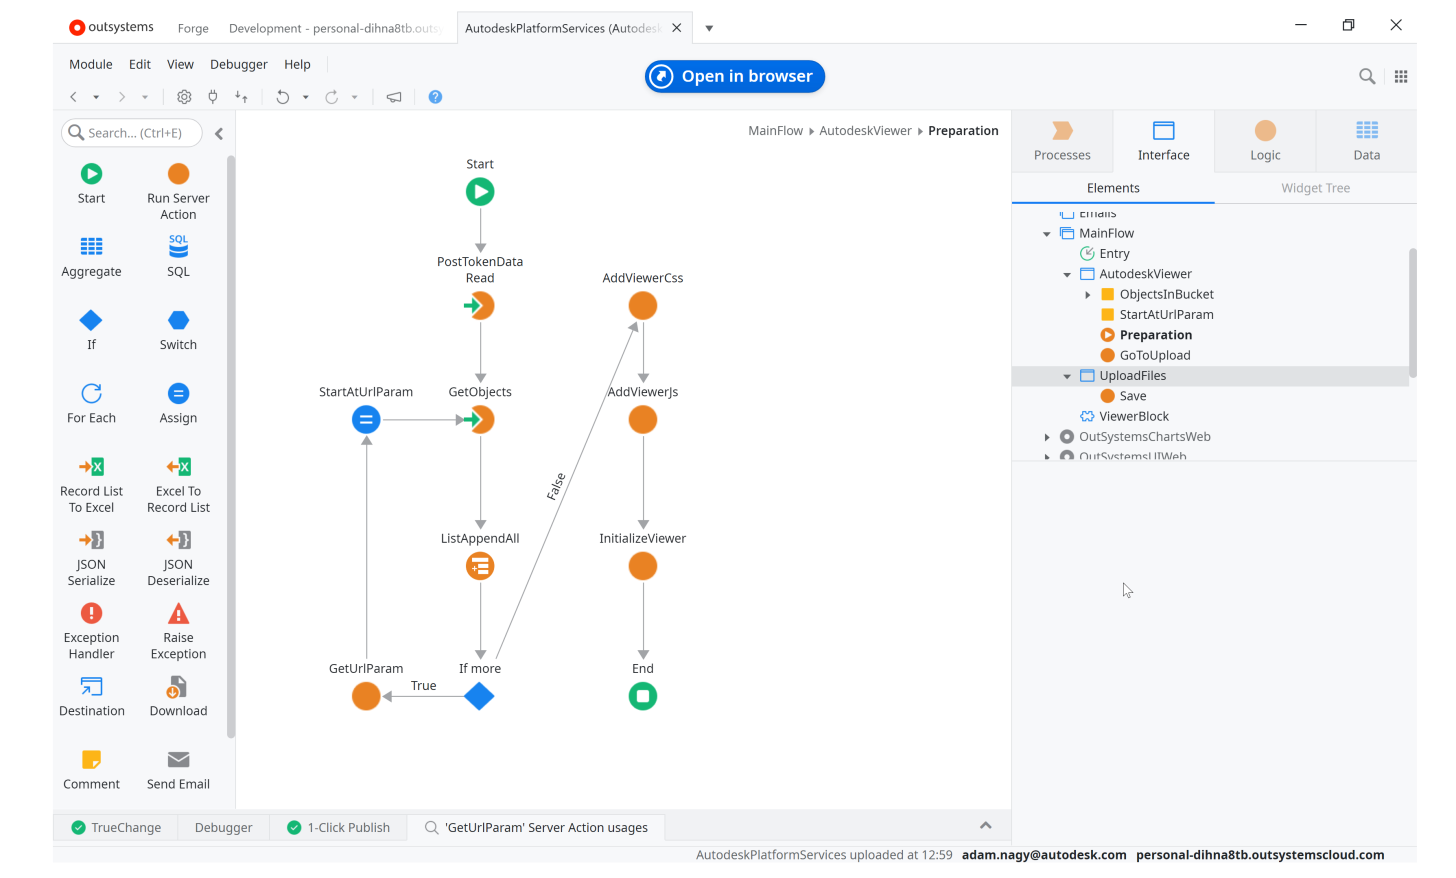
\includegraphics[width=15cm]{Figures/outsystems.png}
    \caption{Interface OutSystems}
    \label{fig:my_label} %Optional (If you want to reference the figure in later chapters)
\end{figure}

\begin{itemize}

    \item \textbf{OutSystems} propose des capacités d'intégration robustes avec divers systèmes bancaires, des systèmes existants et des applications tierces, permettant un flux de données et une interopérabilité transparents. La plateforme offre également des fonctionnalités de sécurité de niveau entreprise, notamment la gestion des identités, le chiffrement et la conformité aux normes du secteur telles que le RGPD et le PCI-DSS. Conçu pour l'évolutivité, OutSystems garantit que les solutions bancaires puissent croître en fonction des besoins de l'institution. Ses outils de création d'interfaces utilisateur riches et réactives améliorent l'expérience client sur les plateformes web et mobiles. Les applications développées à l'aide d'OutSystems incluent des processus d'intégration numérique simplifiés, des flux de traitement et d'approbation de prêts automatisés, ainsi que des applications bancaires mobiles riches en fonctionnalités.



          \begin{figure}[H]
              \centering
              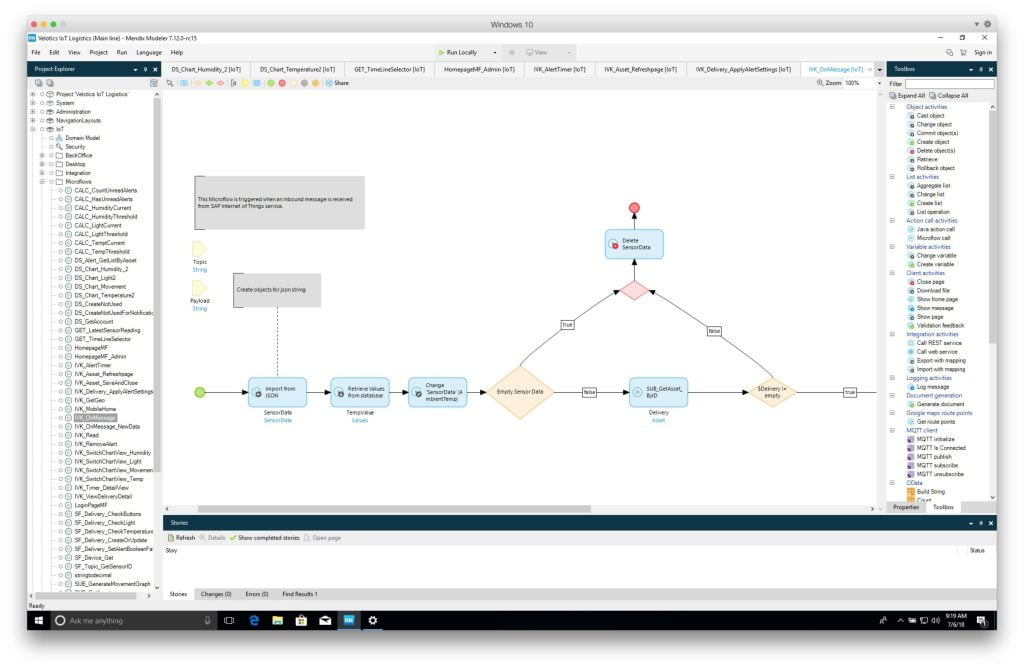
\includegraphics[width=15cm]{Figures/mendix.jpg}
              \caption{Interface Mendix}
              \label{fig:my_label} %Optional (If you want to reference the figure in later chapters)
          \end{figure}


    \item \textbf{Mendix} se concentre sur le développement piloté par modèle, permettant aux utilisateurs de créer des applications à l'aide de modèles visuels. Cela facilite la participation des analystes métier et des non-développeurs au processus de développement. Mendix propose des outils de collaboration complets qui favorisent la coopération entre les équipes informatiques et commerciales, garantissant ainsi que les applications répondent aux exigences de l'entreprise. Grâce à son développement piloté par l'IA, Mendix suggère des bonnes pratiques et optimise les performances des applications. La plateforme fournit également des connecteurs et des API prédéfinis pour l'intégration avec les systèmes bancaires centraux, les plateformes CRM et d'autres applications d'entreprise. Les applications construites avec Mendix incluent des solutions CRM personnalisées adaptées aux besoins spécifiques des banques, des applications de conformité réglementaire pour KYC (Know Your Customer) et AML (Anti-Money Laundering), et des flux de travail internes pour les pistes d'audit, la gestion des risques et les rapports financiers.



          \begin{figure}[H]
              \centering
              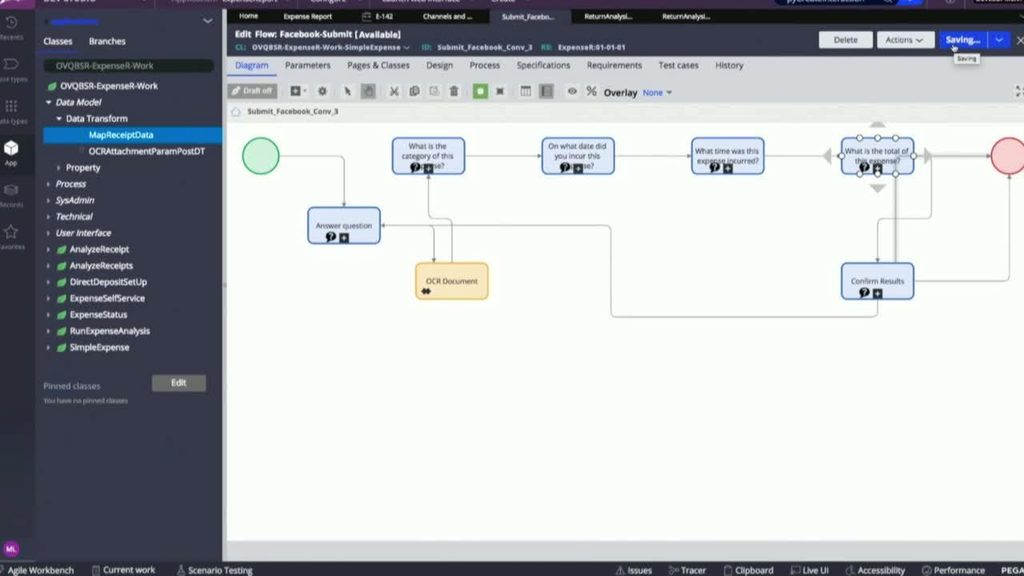
\includegraphics[width=15cm]{Figures/pega.jpg}
              \caption{Interface Pega}
              \label{fig:my_label} %Optional (If you want to reference the figure in later chapters)
          \end{figure}

    \item \textbf{Pega} est reconnu pour ses puissantes fonctionnalités de BPM (Business Process Management) et d'engagement client. Il aide les banques à automatiser les workflows et à gérer plus efficacement les interactions clients. La plateforme Pega intègre une prise de décision pilotée par l'IA, ce qui permet d'améliorer la personnalisation des services proposés aux clients. Les applications développées avec Pega incluent des processus d'intégration client automatisés, des assistants virtuels intelligents pour les demandes des clients et une gestion dynamique des cas pour traiter les demandes et les problèmes clients complexes.


          \begin{figure}[H]
              \centering
              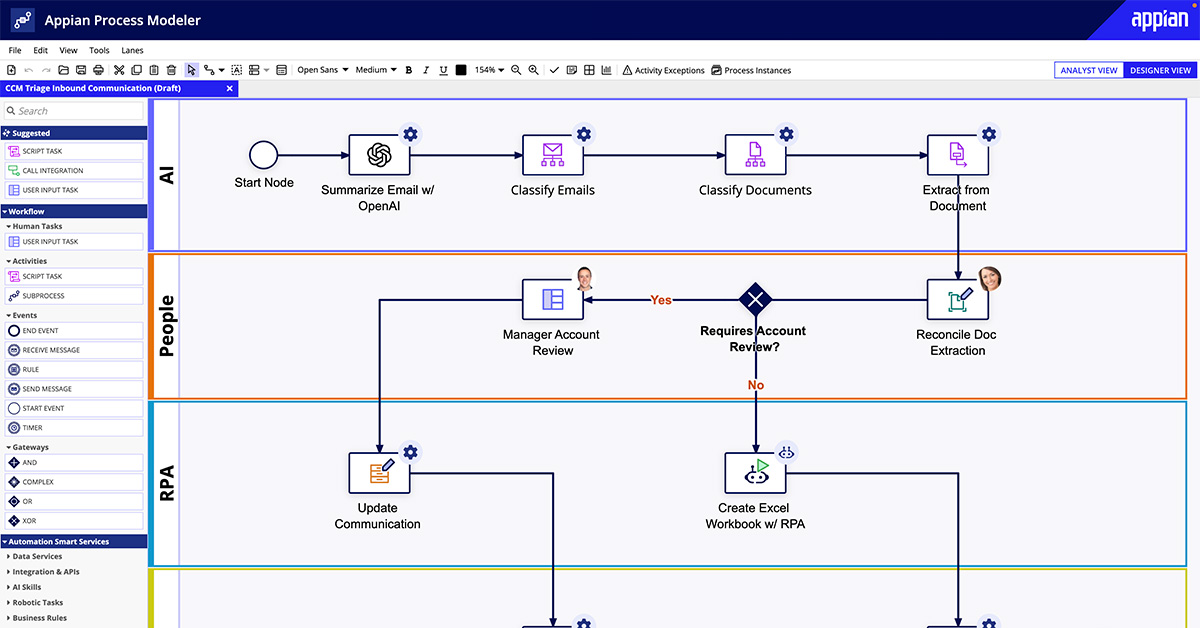
\includegraphics[width=15cm]{Figures/appian.jpg}
              \caption{Interface Appian}
              \label{fig:my_label} %Optional (If you want to reference the figure in later chapters)
          \end{figure}


    \item \textbf{Appian} est une autre plateforme low-code puissante, particulièrement axée sur la gestion des processus métier (BPM). Elle permet aux banques d'automatiser et d'optimiser des processus complexes, en s'intégrant aux outils d'automatisation robotisée des processus (RPA) pour réduire les efforts manuels et les erreurs. Les capacités avancées de gestion des données d'Appian offrent une vue unifiée des données clients, permettant une meilleure prise de décision. Ses outils de gestion de cas améliorent la prestation de services et la satisfaction client. Les applications développées à l'aide d'Appian incluent des systèmes de détection de fraude en temps réel basés sur l'apprentissage automatique et l'analyse, des améliorations du service client telles que des chatbots et des centres de service, ainsi que des solutions de gestion des risques garantissant la conformité aux exigences réglementaires.
\end{itemize}



En résumé, les plateformes low-code révolutionnent le paysage du développement logiciel dans de nombreux secteurs. En permettant le développement et le déploiement rapides d'applications, ces plateformes donnent aux organisations les moyens d'innover et de s'adapter rapidement à l'évolution du paysage numérique. Des plateformes comme OutSystems, Mendix, Appian et Pega se démarquent, mais d'autres acteurs importants existent également dans l'espace low-code, tels que Zoho Creator, Betty Blocks, Quick Base, Kissflow et Bubble. Ces plateformes offrent des fonctionnalités et des capacités diverses qui répondent à un large éventail de besoins opérationnels, de l'automatisation des workflows à l'amélioration de l'engagement client, en passant par l'augmentation de la productivité et la garantie de conformité.  Globalement, les plateformes low-code démocratisent le développement d'applications, le rendant accessible à un public plus large et accélérant considérablement le processus de transformation numérique pour de nombreuses organisations.

\subsection{Content Management System (CMS)}


\hspace{\parindent}Les systèmes de gestion de contenu (CMS) sont des outils essentiels pour gérer, créer et modifier du contenu numérique. Ces systèmes sont devenus indispensables pour les entreprises de toutes tailles, permettant une gestion efficace des sites web, blogs et autres plateformes numériques sans nécessiter de connaissances techniques approfondies.

Un CMS est une application logicielle qui permet aux utilisateurs de créer, éditer, organiser et publier du contenu numérique. Il fournit une interface conviviale pour gérer le contenu web et prend souvent en charge plusieurs utilisateurs dans un environnement collaboratif. L'objectif principal d'un CMS est de simplifier le processus de création de contenu, permettant ainsi aux utilisateurs non techniques de contribuer et de gérer efficacement le contenu numérique.

\textbf{A. Importance des CMS}

Les systèmes de gestion de contenu (CMS) simplifient la gestion du contenu numérique au sein d'une organisation, garantissant une présence en ligne constante et efficace. Les avantages clés incluent :

\begin{itemize}
    \item \textbf{Facilité d'utilisation}: La majorité des CMS disposent d'interfaces conviviales permettant la création et la manipulation de contenu sans connaissances en HTML, CSS ou tout autre langage de programmation utilisé dans le design web.

    \item \textbf{Collaboration}: Ils permettent la collaboration de plusieurs utilisateurs. Des rôles peuvent être créés et assignés, certains utilisateurs ayant plus d'accès et de permissions que d'autres.


    \item \textbf{Efficacité}: En consolidant la gestion du contenu, ils réduisent le temps et les efforts nécessaires pour maintenir les sites web et autres formes de contenu numérique.

    \item \textbf{Scalabilité}: Grâce à leur architecture flexible, ils peuvent gérer un volume important de contenu et de trafic, ce qui les rend adaptés aux entreprises de toutes tailles.

    \item \textbf{Optimisation SEO}: La plupart des plateformes CMS intègrent des outils et plugins tiers pour aider à l'optimisation du contenu pour les moteurs de recherche, augmentant ainsi la visibilité et le classement du contenu.
\end{itemize}

\textbf{B. Fonctionnalités des CMS}


Les plateformes CMS offrent une gamme de fonctionnalités visant à simplifier la gestion du contenu et à améliorer la fonctionnalité :


\begin{itemize}
    \item \textbf{Éditeur WYSIWYG}: Un éditeur \textit{"What You See Is What You Get"} permet aux utilisateurs de créer et formater du contenu avec une interface visuelle affichant l'apparence finale du contenu sur le site web.

    \item \textbf{Templates et Thèmes}: Ils proposent une variété de templates et thèmes préconçus, personnalisables pour correspondre à l'image de marque et au style de l'organisation.

    \item \textbf{Plugins et Extensions}: Ces modules complémentaires étendent la fonctionnalité du CMS, permettant des fonctionnalités telles que le commerce électronique, l'intégration aux réseaux sociaux et l'analyse.

    \item \textbf{Planification du Contenu}: Les utilisateurs peuvent programmer la publication de contenu à des moments précis, facilitant la planification et la gestion des publications.
    \item \textbf{Media Management}: Ils offrent des outils pour télécharger, organiser et gérer les fichiers multimédias tels que les images, vidéos et documents.

    \item \textbf{Gestion des Utilisateurs}: Ils prennent en charge le contrôle d'accès basé sur les rôles, permettant aux administrateurs de gérer les permissions et les niveaux d'accès des utilisateurs.
\end{itemize}

\textbf{C. Exemples et Applications}

Les CMS (Systèmes de Gestion de Contenu) sont largement employés dans divers secteurs, chacun présentant des besoins et des applications spécifiques. Parmi les exemples populaires, on trouve WordPress, Drupal, Joomla et SITECORE.
\begin{figure}[H]
    \centering
    
\includegraphics[width=6cm]{Figures/WordPress.png}
    \caption{WordPress logo}
    \label{fig:my_label} %Optional (If you want to reference the figure in later chapters)
\end{figure}

\begin{itemize}

    \item \textbf{WordPress} est l'un des systèmes de gestion de contenu (SGC) les plus populaires, reconnu pour son interface conviviale, sa vaste bibliothèque de thèmes et de plugins, et son solide support communautaire. Il convient à une large gamme d'applications, des blogs et sites web personnels aux sites d'entreprise et aux plateformes e-commerce.  La simplicité d'utilisation de WordPress pour le référencement (SEO) et sa flexibilité en font un choix de premier plan pour de nombreuses organisations.
          \\
          \\
          \begin{figure}[H]
              \centering
              
\includegraphics[width=5cm]{Figures/Drupal.png}
              \caption{Drupal logo}
              \label{fig:my_label} %Optional (If you want to reference the figure in later chapters)
          \end{figure}


    \item \textbf{Drupal} est un autre système de gestion de contenu (SGC), plébiscité pour sa haute personnalisation, sa scalabilité et ses fonctionnalités de sécurité robustes. Il est fréquemment utilisé par les agences gouvernementales, les institutions d'enseignement et les grands sites communautaires. Le support multilingue intégré de Drupal et ses mesures de sécurité solides en font un choix fiable pour les sites web complexes et à fort trafic.

          \begin{figure}[H]
              \centering
              
\includegraphics[width=7cm]{Figures/Joomla.png}
              \caption{Joomla logo}
              \label{fig:my_label} %Optional (If you want to reference the figure in later chapters)
          \end{figure}


    \item \textbf{Joomla} se positionne comme un juste milieu entre la convivialité et la fonctionnalité avancée. Il propose une large gamme d'extensions et de modèles, prend en charge plusieurs langues et bénéficie d'une communauté de développeurs active. Joomla convient parfaitement aux petites et moyennes entreprises, aux sites e-commerce et aux plateformes de réseaux sociaux.

          \begin{figure}[H]
              \centering
              
\includegraphics[width=5cm]{Figures/Sitecore.png}
              \caption{Sitecore logo }
              \label{fig:my_label} %Optional (If you want to reference the figure in later chapters)
          \end{figure}


    \item \textbf{Sitecore} se démarque par ses outils avancés de gestion de l'expérience client, son intégration transparente avec d'autres systèmes d'entreprise, ses analyses complètes et sa scalabilité. Il est couramment utilisé par les grandes entreprises pour gérer un contenu volumineux et offrir des expériences utilisateur personnalisées. L'intégration de Sitecore avec les outils marketing et sa prise en charge des sites e-commerce complexes en font une solution robuste pour les grandes organisations.

\end{itemize}
\hspace{\parindent}Malgré tous les avantages qu'elles offrent, les plateformes CMS présentent également certains inconvénients. En voici quelques-uns : limitations de la personnalisation, risques de sécurité, problèmes de performance liés aux gros volumes de contenu, et nécessité d'une maintenance et de mises à jour régulières. Les organisations doivent donc tenir compte de ces facteurs lors du choix d'un CMS.

L'avenir des plateformes CMS sera très probablement marqué par l'intégration de l'intelligence artificielle et du machine learning pour améliorer la personnalisation et l'optimisation du contenu. On assistera également à un intérêt accru pour les CMS headless, qui séparent le système de gestion de contenu du back-end de la couche de présentation du front-end, permettant une gestion plus précise de la distribution du contenu sur des plateformes disparates.

Par conséquent, les outils CMS tels que WordPress, Drupal, Joomla, Sitecore et autres sont essentiels pour la gestion de contenu. Ils permettent aux organisations de disposer d'une plateforme en ligne performante, d'interagir avec leur audience et d'évoluer dans l'environnement numérique en constante mutation. Ces plateformes continueront à se développer à mesure des avancées technologiques afin de fournir aux utilisateurs plus de fonctionnalités et de faciliter la gestion du contenu, tout en offrant une meilleure expérience utilisateur.

% \subsection{BPMN}

% \hspace{\parindent}BPMN, ou Business Process Model and Notation (en français, Modélisation et Notation des Processus d'Entreprise), est une méthode standardisée de modélisation graphique des processus d'entreprise. Il offre un moyen complet de cartographier les différentes activités, événements et décisions au sein d'un processus métier, ce qui facilite la compréhension et l'analyse de ces processus par les parties prenantes. BPMN est largement utilisé dans divers secteurs pour améliorer l'efficacité, rationaliser les opérations et garantir la cohérence dans la gestion des processus métier.

% C'est une représentation visuelle permettant de spécifier les processus d'entreprise dans un modèle de processus métier. Il est conçu pour être facilement compréhensible par toutes les parties prenantes de l'entreprise, y compris les analystes métier, qui créent et affinent les processus, les développeurs techniques, responsables de la mise en œuvre des processus et les chefs d'entreprise, qui supervisent et gèrent les processus.

% BPMN utilise un ensemble de symboles normalisés pour représenter les différents aspects d'un processus métier. Ces symboles se répartissent en plusieurs catégories :
% \\
% \begin{figure}[H] 
%     \centering
%     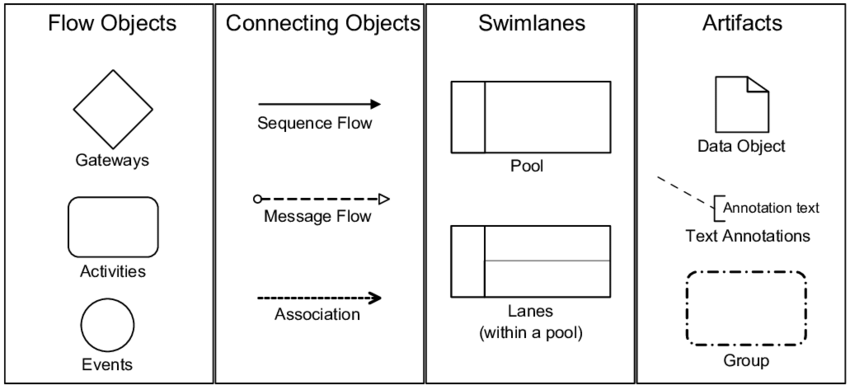
\includegraphics[width=15cm]{Figures/BPMN.png}
%     \caption{BPMN Core Elements of Process diagram}
%     \label{fig:my_label} %Optional (If you want to reference the figure in later chapters)
% \end{figure}

% \\

% \begin{itemize}
% \item \textbf{Flow Objects} 
%     \begin{itemize}
%       \item \textbf{Events} : Represent things that happen (start, intermediate, and end events).
%       \item \textbf{Activities} : Work or tasks performed (tasks, sub-processes).
%       \item \textbf{Gateways} : Decision points that determine the flow of the process (e.g., exclusive, parallel).
%     \end{itemize}

% \item \textbf{Connecting Objects} 
%     \begin{itemize}
%       \item \textbf{Sequence Flows}: Show the order of activities.
%       \item \textbf{Message Flows}: Represent the flow of messages between separate process participants.
%       \item \textbf{Associations}: Link artifacts and text to flow objects.
%     \end{itemize}

% \item \textbf{Swimlanes} 
%     \begin{itemize}
%       \item \textbf{Pools}: Represent major participants in the process.
%       \item \textbf{Lanes}: Sub-divisions within pools that organize and categorize activities.
%     \end{itemize}

% \item \textbf{Artifacts} 
%     \begin{itemize}
%       \item \textbf{Data Objects}: Represent data required or produced by activities.
%       \item \textbf{Groups}: Used to group elements of a diagram informally.
%       \item \textbf{Annotations}: Provide additional information about the process.
%     \end{itemize}

% \end{itemize}


% \hspace{\parindent}BPMN is a crucial tool for businesses aiming to document, analyze, and enhance their processes. By offering a standardized and visual representation, it facilitates better communication, deeper understanding, and continuous improvement across diverse sectors. As organizations embrace digital transformation, it will remain integral to effective process management. In the following sections, we will delve into the various BPMN symbols in detail and examine their application in Fawri-Flows, demonstrating the practical use of this powerful notation system.



\subsection{Présentation de Fawri-Flow}


\hspace{\parindent}Fawri-Flow est un outil de Gestion Intelligente des Processus Métier (IBPM) associé à un moteur de rendu frontal d'écrans. Il permet la transformation et la digitalisation efficaces de divers types de processus, tout en offrant un niveau élevé de personnalisation en termes de design et d'expérience utilisateur (UX).

Fawri-Flow permet d'adapter dynamiquement tout changement ad hoc dans le modèle ou la procédure en modifiant le schéma du processus ou le formulaire de chaque nœud du processus.

La conception des flux de travail repose principalement sur des nœuds de divers types, chacun étant attribué à un rôle spécifique ou suivant une matrice d'approbation configurable :

\begin{itemize}
    \item \textbf{Tâche utilisateur}: Il s'agit d'une page de formulaire ou d'un ensemble de pages attribuées à un rôle spécifique (par exemple : utilisateur final ou agent de traitement).

    \item \textbf{Tâches système ou connecteur}: Permettent l'exécution fluide d'un script grâce à l'éditeur intelligent de la solution.
    \item \textbf{Passerelles}: Ces éléments permettent au dossier ou à la demande de suivre un ou plusieurs chemins en fonction d'un ensemble de conditions entièrement paramétrables, basées sur les données fournies par l'utilisateur ou calculées par le système.
\end{itemize}

Fawri-Flow dispose également d'un Flow Designer, un module d'automatisation des processus dans un environnement de conception graphique. Il permet aux propriétaires de processus d'utiliser le langage naturel pour automatiser les approbations, les tâches, les notifications et les opérations d'enregistrement sans nécessiter de codage.

Flow Designer offre plusieurs avantages : il consolide diverses capacités d'automatisation dans une seule interface, permettant ainsi aux utilisateurs de visualiser et de gérer les processus métier de manière intuitive. Il fournit des descriptions en langage naturel pour faciliter la compréhension des non-techniciens et favorise l'automatisation en permettant aux experts métier de créer et partager des actions réutilisables, ce qui réduit les coûts de développement et de mise à niveau.

\begin{figure}[H]
    \centering
    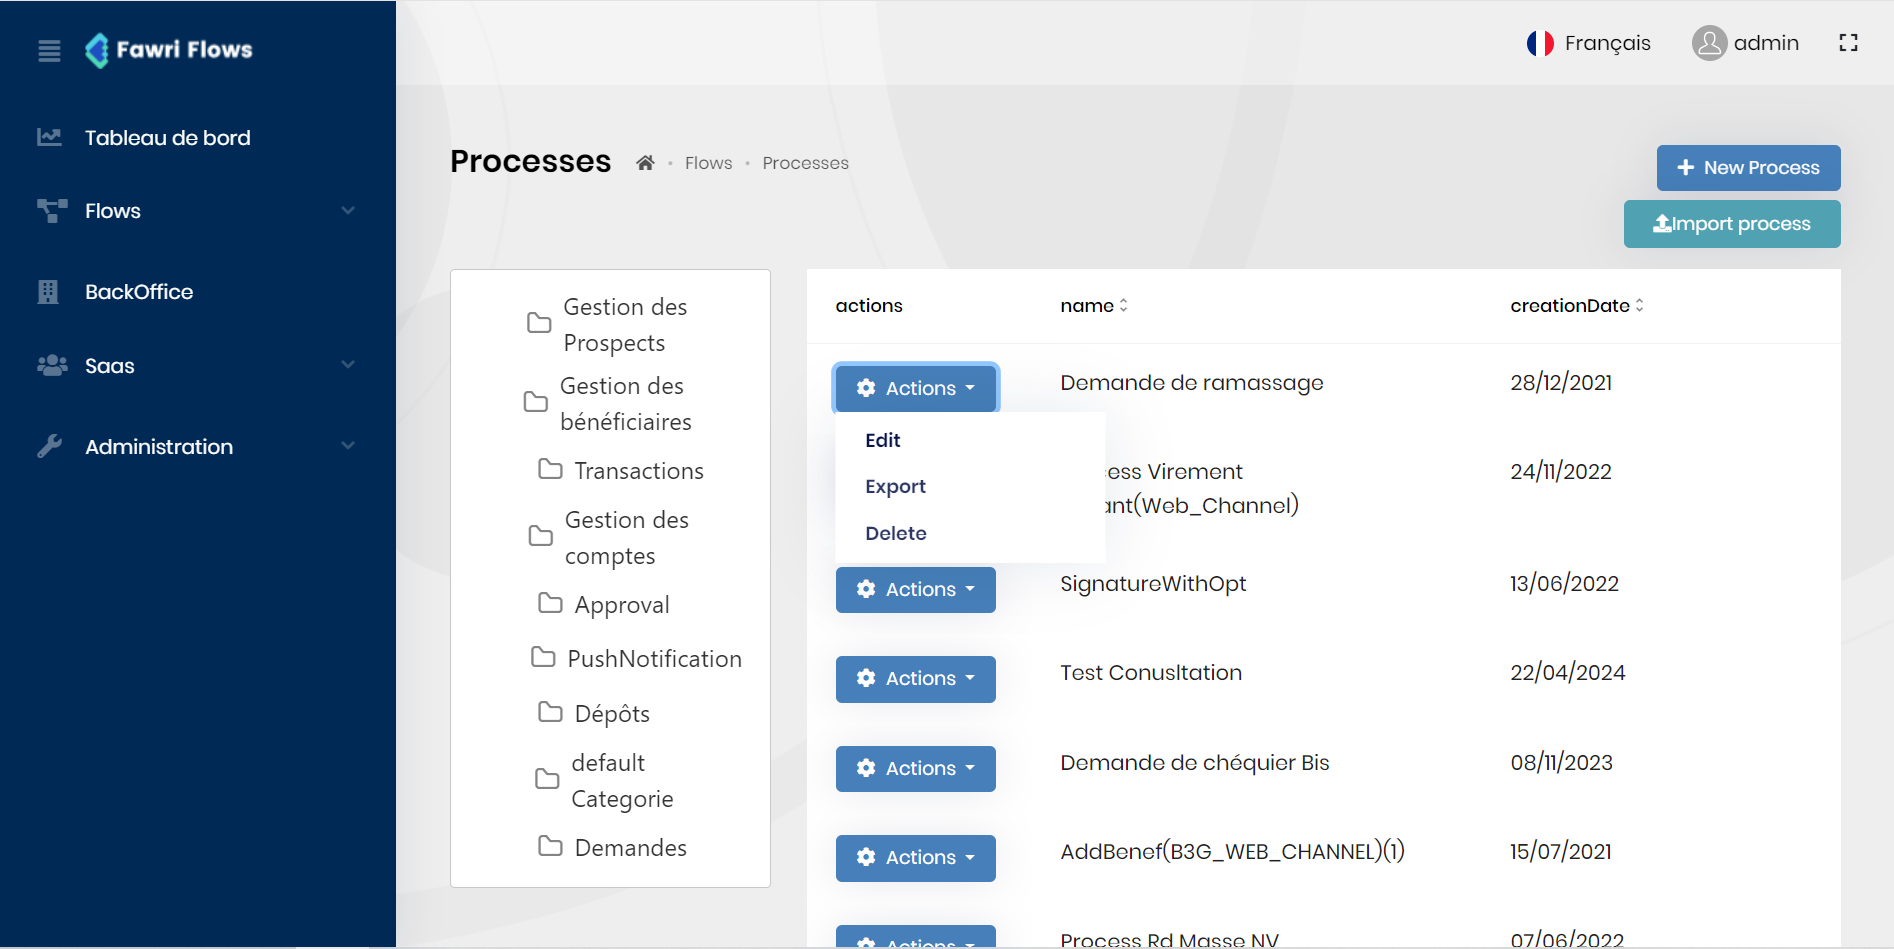
\includegraphics[width=15cm]{Figures/processmanagement.png}
    \caption{Gestion des processus avec Fawri-Flows}
    \label{fig:my_label} %Optional (If you want to reference the figure in later chapters)
\end{figure}



\section{Problématique }

\hspace{\parindent}Bien que Fawri-Flow permette la création de processus intégrables et réutilisables, son intégration actuelle exige une manipulation directe du code. Cette approche engendre d'importantes inefficacités dans le développement des applications clientes, nécessitant des efforts manuels pour coder des composants spécifiques. Cela non seulement consomme davantage de temps et de ressources, mais limite également la capacité à réutiliser efficacement les fonctionnalités existantes et à les adapter aux besoins évolutifs des applications. En outre, en dehors de l'intégration des processus, le développement complet de l'application pour chaque client doit être réalisé. Cette dépendance à la programmation manuelle des composants entrave le processus de développement, compromettant ainsi la productivité et la rentabilité du projet.

Face à cette situation, se pose la question suivante : \textbf{Comment évoluer vers une solution low-code qui simplifie le processus de développement d'applications, en exploitant pleinement les capacités de Fawri-Flow, tout en éliminant le besoin de manipulation directe du code ?}

\section{Objectifs du Projet et Solutions Proposées}

\hspace{\parindent}B3G a voulu lancer \textbf{Fawri-CMS}, une nouvelle solution alignée sur la tendance du "low-code". L'objectif principal de ce projet est de simplifier considérablement le processus de développement des applications clientes, notamment dans les secteurs du \textit{digital banking} et des portefeuilles numériques, en éliminant la nécessité de recourir à la programmation traditionnelle. Avec une interface conviviale de type "drag and drop", Fawri-CMS facilitera également l'intégration des processus métier élaborés avec Fawri-Flows.

Ce nouvel outil vise plusieurs objectifs stratégiques. Tout d'abord, il cherche à réduire drastiquement le temps et les ressources nécessaires au développement des applications, en supprimant la phase de codage manuel pour chaque fonctionnalité. En rendant possible la création d'applications professionnelles et fonctionnelles même pour un public non spécialisé en programmation, Fawri-CMS aspire à démocratiser l'accès au développement d'applications. De plus, il entend améliorer l'efficacité opérationnelle des entreprises en facilitant une intégration fluide des processus métier dans les applications clientes, même sans compétences techniques approfondies. Enfin, en libérant les développeurs des contraintes techniques, Fawri-CMS encourage l'innovation et la créativité, en les incitant à se concentrer sur la conception et l'expérience utilisateur.




\section{Gestion du projet}

\subsection{Approche Scrum}

\hspace{\parindent}Dans le choix de la méthodologie pour ce projet, plusieurs facteurs ont influencé notre décision, notamment les exigences spécifiques du projet, sa nature et ses objectifs. La méthodologie Scrum s'est imposée comme le cadre le plus adapté pour répondre à ces besoins. Voici les principaux éléments de Scrum :

\textbf{Rôles :}


\begin{itemize}
    \item \textbf{Product Owner} : Responsable de définir et prioriser le backlog du produit, déterminer les fonctionnalités à développer et garantir la valeur du produit.

    \item \textbf{Scrum Master} : Facilitateur du processus Scrum, s'assurant que l'équipe respecte les principes et pratiques de Scrum et résout les obstacles éventuels.

    \item \textbf{Équipe de développement} : Groupe de personnes responsables de réaliser les fonctionnalités du produit. Dans le cadre de ce projet, nous faisons partie de cette équipe et sommes responsables de sa réalisation.
\end{itemize}



\textbf{Artéfacts :}


\begin{itemize}
    \item \textbf{Product Backlog} : Liste ordonnée des fonctionnalités à développer, représentant les besoins et exigences du produit.

    \item \textbf{Sprint Backlog} :Liste des fonctionnalités sélectionnées à partir du Product Backlog pour être développées lors d'un sprint spécifique.

    \item \textbf{Increment} : Version fonctionnelle du produit résultant des fonctionnalités développées pendant un sprint.
\end{itemize}


\textbf{Événements :}


\begin{itemize}
    \item \textbf{Sprint} : Période de temps définie (généralement de 1 à 4 semaines) au cours de laquelle l'équipe de développement crée un incrément de produit.

    \item \textbf{Sprint Planning} : Réunion de planification où l'équipe sélectionne les fonctionnalités à développer pendant le sprint et détermine comment les réaliser.

    \item \textbf{Daily Scrum} : Réunion quotidienne de l'équipe pour partager les progrès, synchroniser les activités et discuter des obstacles éventuels.

    \item \textbf{Sprint Review} : Réunion à la fin du sprint pour présenter l'incrément du produit aux parties prenantes et recueillir des commentaires.

    \item \textbf{Sprint Retrospective} : Réunion pour réfléchir sur le sprint écoulé, identifier les points forts et les améliorations possibles, et adapter les pratiques.


\end{itemize}


La nature itérative et incrémentielle de Scrum correspondait parfaitement à la volonté d'optimiser la gestion du projet et la collaboration au sein de notre équipe. Face à un projet dynamique et évolutif tel que celui-ci, Scrum offrait la flexibilité nécessaire pour s'adapter aux changements tout en garantissant des livraisons régulières de fonctionnalités.

De plus, la structure claire des rôles, des artefacts et des événements de Scrum nous permettait de définir des responsabilités précises et de favoriser la transparence tout au long du processus de développement. Cette clarté était essentielle pour assurer une communication efficace au sein de l'équipe et avec les parties prenantes externes.

En adoptant Scrum, nous avons pu bénéficier d'une approche collaborative et adaptative, permettant à notre équipe de rester focalisée sur la valeur à apporter au produit tout en s'assurant d'une progression constante. La méthodologie Scrum a ainsi joué un rôle crucial dans le succès de notre projet, en fournissant un cadre solide pour la gestion de projet agile et en favorisant la collaboration, la responsabilisation et l'amélioration continue.


\begin{figure}[H]
    \centering
    
\includegraphics[width=4cm]{Figures/scrum.png}
    \caption{Scrum logo}
    %\label{fig:my_label} %Optional (If you want to reference the figure in later chapters)
\end{figure}








\subsection{Outils de collaboration}

\hspace{\parindent}Pour améliorer l'efficacité et la productivité au sein de l'équipe B3G, l'intégration d'outils collaboratifs s'est avérée indispensable. Nous nous sommes concentrés sur deux outils déjà en usage avant le début du stage : \textbf{Microsoft Teams} et \textbf{Outlook}. Microsoft Teams est devenu un élément central de notre collaboration. En créant des espaces de travail dédiés à chaque projet ou équipe, nous avons pu regrouper les discussions, les partages de fichiers et les réunions, facilitant ainsi une communication fluide et une organisation optimale des tâches.

Les fonctionnalités de chat, d'appels audio et vidéo de Teams ont été d'une grande utilité pour maintenir une communication efficace et instantanée, quel que soit l'emplacement géographique des membres de l'équipe. De plus, les partages d'écran se sont avérés particulièrement utiles lors des réunions pour présenter des informations clés ou réaliser des démonstrations.\\

\begin{figure}[H]
    \centering
    
\includegraphics[width=6cm]{Figures/Microsoft_Teams.png}
    \caption{Microsoft Teams logo}
    %\label{fig:my_label} %Optional (If you want to reference the figure in later chapters)
\end{figure}


Outlook, de son côté, a été utilisé pour la gestion des calendriers et la planification. Nous avons pu créer des rendez-vous, des réunions et des rappels directement dans Outlook, ce qui nous a permis de structurer nos emplois du temps et d'éviter les conflits d'horaire. Grâce à la fonction de partage de calendrier, nous avons pu visualiser les disponibilités des membres de l'équipe et planifier des réunions aux moments les plus propices. De plus, la fonction d'intégration d'Outlook avec d'autres outils, tels que Teams, nous a facilité la transformation des e-mails en discussions collaboratives, ce qui a favorisé une communication améliorée et une productivité accrue.
\\
\\
\begin{figure}[H]
    \centering
    
\includegraphics[width=6cm]{Figures/outlook.png}
    \caption{Microsoft Oulook logo}
    %\label{fig:my_label} %Optional (If you want to reference the figure in later chapters)
\end{figure}



\subsection{Gestion des versions}

Puisque nous adhérons à la méthodologie agile, une collaboration étroite entre les membres de l'équipe sur le code est cruciale pour garantir la transparence du développement et le succès du projet. C'est pourquoi le choix d'une plateforme de gestion de code adaptée à nos besoins revêtait une importance capitale.

Dans cette optique, notre société a opté pour \textbf{Azure DevOps Server}. Cette plateforme de développement logiciel offre un ensemble complet d'outils pour la collaboration, le suivi des problèmes, la gestion des versions et le déploiement continu. Elle permet à notre équipe de travailler de manière synchronisée et efficace, en mettant l'accent sur la transparence et la qualité du code.
\\
\\
\begin{figure}[H]
    \centering
    
\includegraphics[width=8cm]{Figures/azur.png}
    \caption{Microsoft Azur DevOps logo}
    %\label{fig:my_label} %Optional (If you want to reference the figure in later chapters)
\end{figure}


\subsection{Planning du projet}

\hspace{\parindent}Dans ce projet, nous avons adopté la planification par sprint avec Scrum, qui fait partie de la méthodologie agile. Cette approche repose sur des cycles itératifs et incrémentaux appelés sprints, généralement d'une durée de 2 à 4 semaines. Elle offre une visualisation claire et pratique des actions planifiées, permettant de suivre et de contrôler le déroulement de chaque étape du projet. Ce diagramme représente graphiquement les tâches et leur durée. Pour ce projet de fin d’études, la figure suivante présente la planification par sprints, offrant une vue d'ensemble de la planification anticipée des tâches. Grâce à cette visualisation, nous pouvons gérer efficacement les échéances et assurer le bon déroulement du projet en respectant les délais fixés.

\begin{figure}[H]
    \centering
    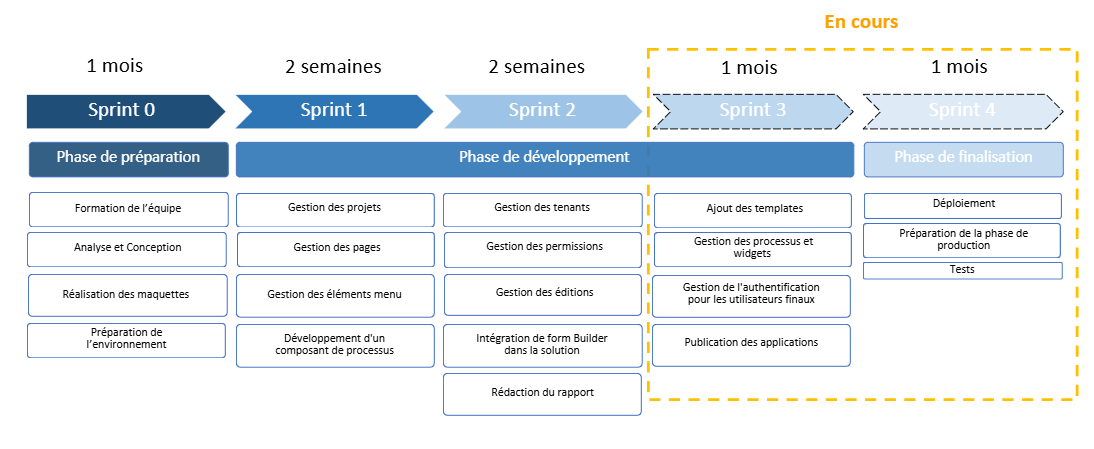
\includegraphics[width=18cm]{Figures/sprints.PNG}
    \caption{Planning du Projet par Sprints}
    %\label{fig:my_label} %Optional (If you want to reference the figure in later chapters)
\end{figure}



\newpage

\section*{Conclusion}

\hspace{\parindent}Dans ce chapitre, nous avons commencé par présenter B3G, une entreprise spécialisée dans le développement de solutions digitales pour le secteur bancaire, en mettant en avant ses produits et sa clientèle. Ensuite, nous avons examiné le contexte global de notre projet, mettant en évidence l'importance croissante de la transformation digitale, ainsi que des concepts clés tels que la technologie "Low-Code", les systèmes de gestion de contenu (CMS), et notre produit Fawri-Flow. Nous avons ensuite défini clairement la problématique de notre projet, suivi par la définition de ses objectifs et des solutions proposées. Nous avons également décrit en détail notre approche méthodologique basée sur Scrum, les outils de collaboration et de gestion des versions utilisés, ainsi que la planification prévisionnelle du projet.

